\documentclass{beamer}
\usepackage{amsmath, amssymb}
\usepackage{graphicx}
\usepackage{hyperref}
\usepackage{listings}
\usepackage{xcolor}
\usepackage[utf8]{inputenc}

\usetheme{Madrid}
\usecolortheme{default}

\setbeamersize{text margin left=1.5cm}
\setbeamersize{text margin right=1.5cm}
\setbeamersize{sidebar width left=0pt}
\setbeamersize{sidebar width right=0pt}

\title{Probabilistic optimization in manufacturing}
\subtitle{Simulated Annealing meets Set Packing}
\author{Michal Racko \\ PyCon PL 2025}
\date{August 30, 2025}

\lstset{
    language=Python,
    basicstyle=\ttfamily\tiny,
    keywordstyle=\color{blue},
    commentstyle=\color{gray},
    stringstyle=\color{red},
    showstringspaces=false,
    breaklines=false,
    breakatwhitespace=true,
    frame=single,
    frameround=tttt,
    framesep=5pt,
    columns=fullflexible,
    keepspaces=true,
    literate={>>>}{{\textcolor{red}{>\!>\!>}}}3
             {...}{{\textcolor{red}{.\!.\!.}}}3
}

\begin{document}

\begin{frame}
  \titlepage
\end{frame}

\begin{frame}{Outline}
  \tableofcontents
\end{frame}

\section{Introduction}

\begin{frame}{What are Monte Carlo methods?}
  \begin{itemize}
    \item Statistical techniques using random sampling
    \item Solve problems that are impossible or impractical to solve analytically
    \item Key principle: Use randomness to approximate deterministic results
  \end{itemize}
  
  \vspace{0.5cm}
  \textbf{Applications:}
  \begin{itemize}
    \item Physics simulations
    \item Financial modeling
    \item Machine learning
    \item Engineering optimization
  \end{itemize}
\end{frame}

\section{Basic concept}

\begin{frame}{Starting at square one}
  \framesubtitle{Value of $\pi$ can be estimated using random sampling}
  \begin{columns}[c]
    \begin{column}{0.5\textwidth}
      Let's pretend $\pi$ is an unknown constant which has to be estimated.
      \vspace{0.5cm}

      \textbf{Geometric considerations}
      \begin{itemize}
        \item Circle area: $A_{circle} = \pi$
        \item Square area: $A_{square} = 4$
        \item Ratio: $\frac{\pi}{4} = \frac{A_{circle}}{A_{square}}$
      \end{itemize}
      
      \vspace{0.5cm}
      Therefore: $\pi = 4 \times \frac{A_{circle}}{A_{square}}$
    \end{column}
    \begin{column}{0.5\textwidth}
      \begin{center}
        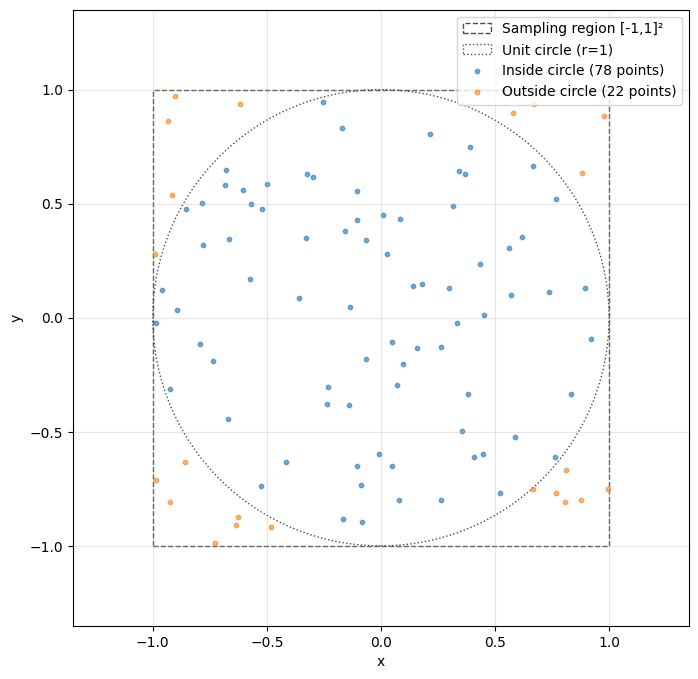
\includegraphics[width=\textwidth]{images/unit_circle_diagram.png}
        \\[0.2cm]
        \small{Unit circle inscribed in square}
      \end{center}
    \end{column}
  \end{columns}
\end{frame}

\begin{frame}{Starting at square one}
\framesubtitle{Value of $\pi$ can be estimated using random sampling}
  \textbf{Key Insight:} All random points are uniformly distributed in the square

  \begin{itemize}
    \item Point $(x,y)$ is \textcolor{blue}{inside} circle if: $x^2 + y^2 \leq 1$
    \item Point $(x,y)$ is \textcolor{orange}{outside} circle if: $x^2 + y^2 > 1$
  \end{itemize}
  
  \vspace{0.5cm}
  \textbf{Therefore we can estimate}
  $$\pi \approx 4 \times \frac{\text{points inside circle}}{\text{total points}}$$
\end{frame}

\begin{frame}[fragile]{Starting at square one}
\framesubtitle{Value of $\pi$ can be estimated using random sampling}
\begin{lstlisting}
>>> import numpy as np
>>> class MonteCarloSamples:
...     def __init__(self, n_samples: int):
...         # Generate random points in [-1,1] x [-1,1]
...         self._samples = np.random.random((n_samples, 2)) * 2 - 1
...
...     def __len__(self) -> int:
...         return len(self._samples)
...
...     @property
...     def centre_distances(self) -> np.ndarray:
...         return np.sqrt((self._samples ** 2).sum(axis=1))
...     
...     @property
...     def within_unit_circle(self) -> np.ndarray:
...         return self.centre_distances <= 1
...     
...     @property
...     def pi_estimate(self) -> float:
...         return float(self.within_unit_circle.sum() / len(self) * 4)
...
>>> samples = MonteCarloSamples(100)
>>> print(samples.pi_estimate)
3.12
\end{lstlisting}
\end{frame}

\begin{frame}{Starting at square one}
  \framesubtitle{Value of $\pi$ can be estimated using random sampling}
  \begin{columns}[c]
    \begin{column}{0.5\textwidth}
      Adding more random samples improves precision
      \vspace{0.5cm}

      \textbf{Geometric considerations}
      \begin{itemize}
        \item 100 samples: $\pi \approx 3.12$
        \item 5,000 samples: $\pi \approx 3.1680$
        \item 10,000,000 samples: $\pi \approx 3.1408$
      \end{itemize}
    \end{column}
    \begin{column}{0.5\textwidth}
      \begin{center}
        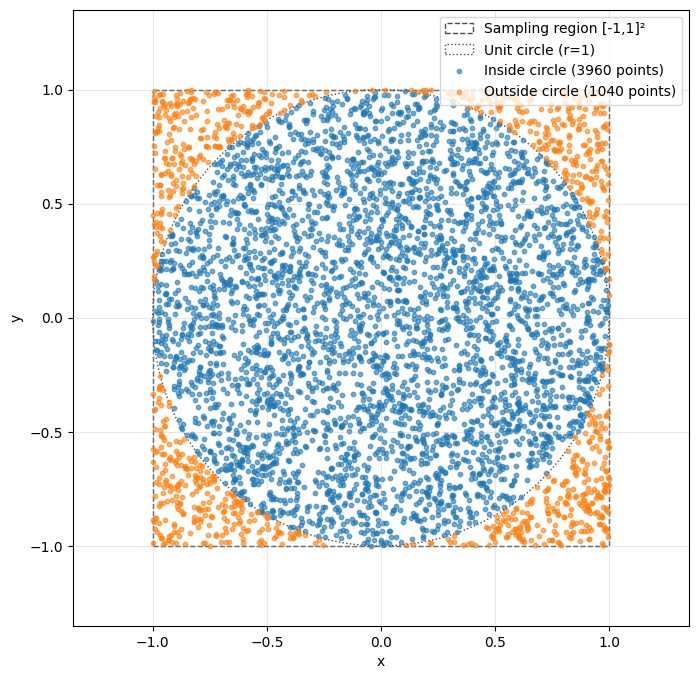
\includegraphics[width=\textwidth]{images/more_samples.png}
        \\[0.2cm]
        \small{More random points drawn from the uniform distribution}
      \end{center}
    \end{column}
  \end{columns}
\end{frame}

\begin{frame}{Starting at square one}
  \framesubtitle{Value of $\pi$ can be estimated using random sampling}

  \begin{columns}[c]
    \begin{column}{0.4\textwidth}
      \textbf{Uncertainty estimation}
      \begin{itemize}
        \item Our estimate follows: $X \sim \text{Binomial}(N, p)$
        \item $\text{Var}(\hat{\pi}) = 16 \cdot \frac{p(1-p)}{N}$
        \item Standard deviation: $\sigma \propto \frac{1}{\sqrt{N}}$
      \end{itemize}
    \end{column}
    \begin{column}{0.6\textwidth}
      \begin{center}
        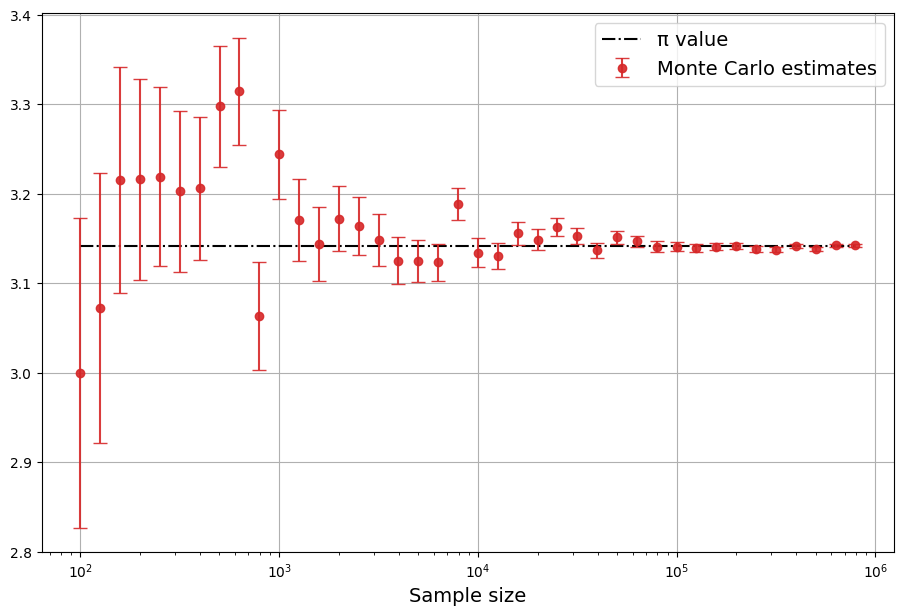
\includegraphics[width=\textwidth]{images/pi_convergence.png}
        \\[0.2cm]
        \small{Monte Carlo estimates converge to the true value as $N \to \infty$}
      \end{center}
    \end{column}
  \end{columns}
\end{frame}

\begin{frame}{Thank You!}
  \begin{center}
    \Large{I'm looking forward to answering your questions}
    
    \vspace{1cm}
    
    \textbf{Key Messages:}
    \begin{itemize}
      \item Monte Carlo methods are powerful for complex problems
      \item Variance reduction techniques can significantly improve efficiency
      \item Measurement without uncertainty is meaningless
    \end{itemize}
  \end{center}
\end{frame}

\end{document}